\subsubsection{Solstrålning genom fönster}

Exempel på resultat från beräkningar på solstrålning genom fönster. Beräknat via trial.m i code-mappen.

\begin{figure}[hpbt]
\centering
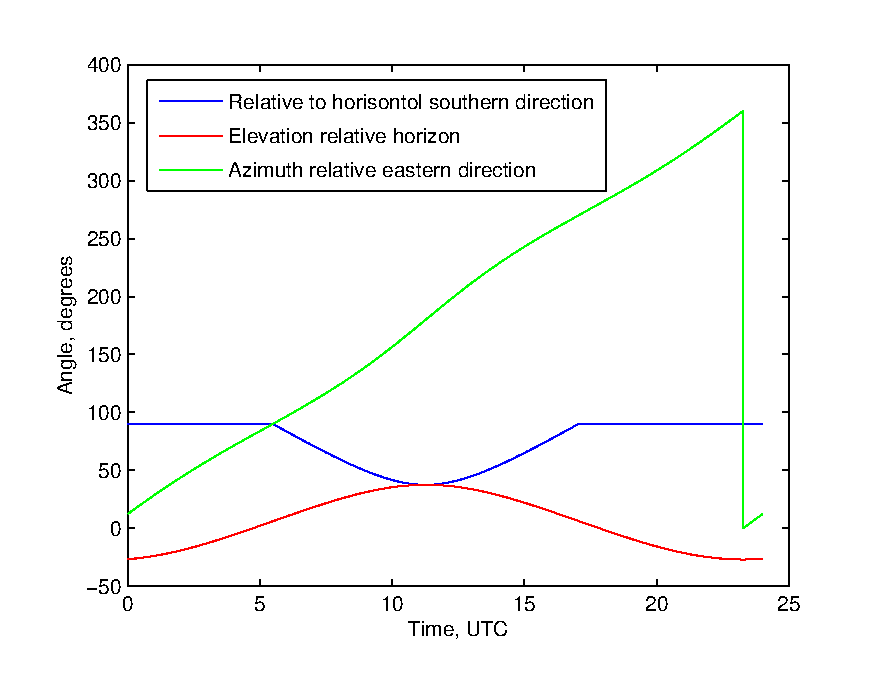
\includegraphics[scale=1]{images/angles120401.eps}
\caption{\label{fig:vinklar120401} Beräknade vinklar vid Walleriusgatan den första april 2012, tid i UTC}
\end{figure}

\begin{figure}[hpbt]
\centering
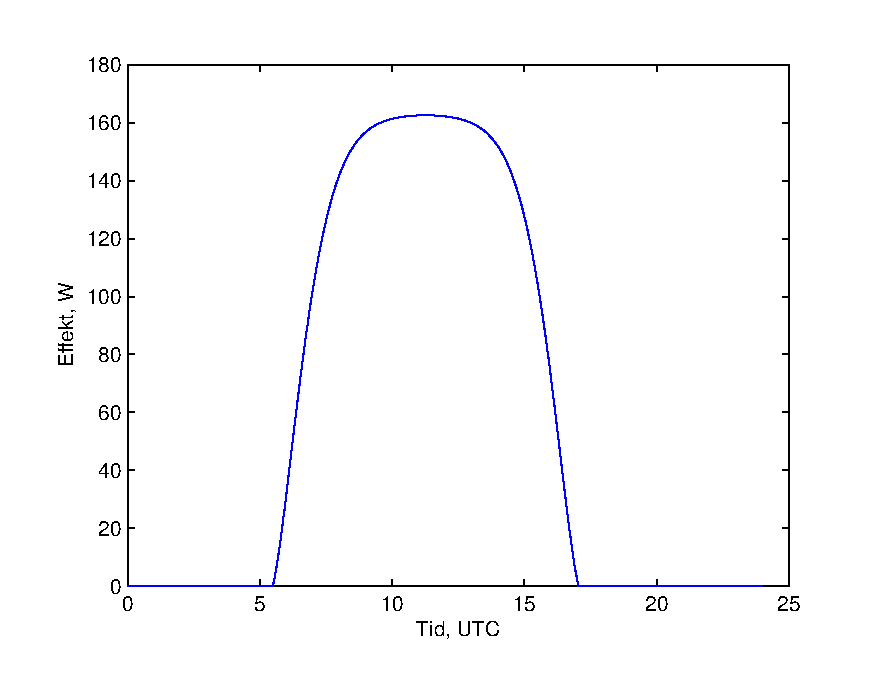
\includegraphics[scale=1]{images/effekt120401.eps}
\caption{\label{fig:effekt120401} Beräknad effekt genom ett fönster vars normal pekar i horisontella sydriktningen, den första april 2012. Solens intensitet tas konstant till 200 W/m$^2$}
\end{figure}
